% !TeX root = analysis.tex
% !TeX program = pdflatex
\documentclass[12pt,a4paper]{article}

% =====================
% Packages
% =====================
\usepackage[top=1in,left=1in,right=1in,bottom=1.6in]{geometry}
\usepackage{array}
\usepackage{ragged2e}
\usepackage{setspace}
\usepackage{hyperref}
\usepackage{enumitem}
\usepackage{graphicx}
\usepackage{eso-pic}  % For background images
\usepackage{fancyhdr}
\usepackage{tabularx}
\usepackage{booktabs}
\usepackage{multirow}
\usepackage{float}
\usepackage{xcolor}
\usepackage{parskip}
\usepackage{amsmath}
\usepackage{wrapfig}
\usepackage{amssymb}
\usepackage{colortbl}
\usepackage{longtable}
\usepackage{textcomp}
\usepackage{caption}
\usepackage{bookmark}
\definecolor{critical}{RGB}{255, 200, 200}
\definecolor{high}{RGB}{255, 230, 200}
\definecolor{medium}{RGB}{255, 255, 200}
\definecolor{tableheader}{RGB}{240, 240, 240}
\definecolor{tablerow}{RGB}{250, 250, 250}
\frenchspacing

% =====================
% Font (pdflatex-friendly Arial-like)
% =====================
\usepackage[T1]{fontenc}
\usepackage[scaled=0.95]{helvet}
\renewcommand{\familydefault}{\sfdefault}

\setstretch{1.2}

% =====================
% BACKGROUND IMAGES SETUP
% =====================
% Cover page (Page 1): Brigman_Letterhead.pdf
% All other pages: Brigman_Paper.pdf

% Background for COVER PAGE ONLY (Page 1)
\AddToShipoutPictureBG*{%
  \AtPageLowerLeft{%
    
\includegraphics[width=\paperwidth,height=\paperheight]{../templates/Brigman_Letterhead.pdf}%
  }%
}

% Background for ALL OTHER PAGES (Page 2 onwards)
\AddToShipoutPictureBG{%
  \ifnum\value{page}>1
    \AtPageLowerLeft{%
      
\includegraphics[width=\paperwidth,height=\paperheight]{../templates/Brigman_Paper.pdf}%
    }%
  \fi
}

% =====================
% Header/Footer (page numbers must appear)
% =====================
\pagestyle{fancy}
\fancyhf{} % clear all
\lhead{\textbf{Brigman Deep Sea Technology}}
\rhead{Software Requirements Analysis (BCIC Methodology)}
\cfoot{\thepage}
\renewcommand{\headrulewidth}{0.4pt}
\setlength{\headheight}{20pt}

\begin{document}

% =====================
% COVER PAGE (Page 1)
% =====================
\thispagestyle{empty}

% Clear all headers for cover page
\fancyhf{}
\lhead{}
\rhead{}
\cfoot{}
\renewcommand{\headrulewidth}{0pt}

% Adjust margins for first page to fit within letterhead
\newgeometry{top=5.2cm,left=1in,right=1in,bottom=1.6in} % Adjust as needed

\begin{center}

\includegraphics[width=0.4\textwidth]{../templates/brigman logo.png}\\[0.5cm]

\LARGE\textbf{Software Requirements Analysis Report}\\[0.5cm]
\large\textbf{Abyss Navigator Suite Project}\\[0.5cm]

\textbf{\Large Brigman Deep Sea Technology}\\
\today
\end{center}
% cover page continues
\fancyhf{} % clear all
\lhead{\textbf{Brigman Deep Sea Technology}}
\rhead{Software Requirements Analysis (BCIC Methodology)}
\cfoot{\thepage}
\renewcommand{\headrulewidth}{0.4pt}
\setlength{\headheight}{20pt}

% =====================
% TABLE OF CONTENTS (Page 2)
% =====================
\newpage
\thispagestyle{empty}
\renewcommand{\contentsname}{Table of Contents}
\tableofcontents

% =====================
% EXECUTIVE SUMMARY (Page 3)
% =====================
\newpage
\setcounter{page}{3}
\section{Executive Summary}
\label{sec:executive}

Brigman Deep Sea Technology completed software requirements analysis for the Abyss Navigator Suite using BCIC, transforming ambiguous inputs into measurable and testable specifications.

Across 27 Project Specification clauses, we identified 15 incongruities (55.6\%) and resolved 86.7\% through targeted stakeholder sessions. Key outputs include quantitative constraints such as 99\% waypoint accuracy, 5-second emergency detection thresholds, and AES-256 security controls.

The regulated-revision process produced codified, verifiable requirements grouped into Navigation, Communication, Safety, and Interface domains. This early analysis is estimated to avoid \$350K+ in rework and reduce schedule risk by 4-6 weeks.

% =====================
% BCIC METHODOLOGY APPLICATION (Pages 5-8)
% =====================
\newpage
\section{BCIC Methodology Application}
\label{sec:bcic}

% ------------------------------------------------------------------
% 2.1 Breakdown Activity – Single Example (BO-L1-4)
% ------------------------------------------------------------------
\subsection{Breakdown Activity: Systematic Incongruity Detection}

The Breakdown activity applies the Incongruous Requirements Checklist (IRC) to each Project Specification clause across Imperative, Continuance, and Contextual checks. This process identified \textbf{15 incongruities} across 27 clauses (55.6\%).

As the primary example, \textbf{BO-L1-4 (Emergency and Abnormal Situation Handling)} triggered three IRC flags. Table~\ref{tab:breakdown-example} summarizes the issue and clarification question raised to the client.

\begin{table}[H]
\centering
\small
\renewcommand{\arraystretch}{1.3}
\caption{IRC Application for Example Requirement BO-L1-4}
\label{tab:breakdown-example}
\begin{tabular}{|>{\raggedright\arraybackslash}p{0.13\textwidth}|>{\raggedright\arraybackslash}p{0.13\textwidth}|>{\raggedright\arraybackslash}p{0.32\textwidth}|c|>{\raggedright\arraybackslash}p{0.3\textwidth}|}
\hline
\rowcolor{tableheader}
\textbf{PS Ref} & \textbf{IRC Flags} & \textbf{Reason} & \textbf{Clarify?} & \textbf{Question for Client} \\
\hline
BO-L1-4 & CTX-1, CTX-2, CON-2 & “Abnormal conditions” undefined, not testable; deferred definition. & Y & What quantitative thresholds define “abnormal conditions” for pressure, temperature, and power deviations? \\
\hline
\end{tabular}
\end{table}

The same IRC process was applied to every clause. The complete set of findings, including all flags and resolutions, is documented in Table~\ref{tab:irc-complete}. By focusing on the most incongruent requirement, we established a repeatable pattern for detecting and documenting issues, ensuring consistent rigor across the entire specification.

\subsection{Clarify Activity: Stakeholder Engagement and Resolution}

\noindent
\textbf{Paper Napkin Sketches as Collaborative Tools.} Prior to the clarification session, our team prepared hand-drawn \textbf{Context} and \textbf{Use Case} diagrams to support rapid stakeholder feedback.

Initial napkin sketches are archived in the project repository and were used as working artifacts during clarification.

During the clarification session, stakeholders annotated these sketches and validated operational boundaries and actors. For \textbf{BO-L1-4}, the client clarified:

\begin{itemize}
    \item Pressure deviation of \(\pm5\%\) sustained for 5 seconds constitutes an “abnormal condition”.
    \item Temperature deviation of \(\pm10\%\) from nominal, and power supply deviation of \(\pm15\%\), are also abnormal thresholds.
    \item Upon detection, the system must automatically transition the submersible to a \textbf{safe operational state}, defined as neutral buoyancy, minimal power consumption, and active communication beacon.
\end{itemize}

These inputs resolved the CTX‑1, CTX‑2, and CON‑2 flags for BO-L1-4 and were replicated across other flagged requirements. Stakeholder feedback indicated a \textbf{40\% reduction in clarification time} versus text-only reviews.

\subsection{Interpret Activity: Regulated-Revision Demonstration}

Following clarification, stakeholder inputs were transformed into precise, measurable, and verifiable software requirements through a \textbf{regulated-revision} process:

\begin{itemize}
    \item \textbf{Imperative issues (IMP):} replace weak or passive phrasing with strong obligations (“shall”).
    \item \textbf{Continuance issues (CON):} decompose compound statements into atomic requirements.
    \item \textbf{Contextual issues (CTX):} insert quantitative thresholds, define ambiguous terms, and add verification methods.
\end{itemize}

\noindent
For our example requirement, the transformation is shown in Table~\ref{tab:interpret-example}.

\begin{table}[H]
\centering
\small
\renewcommand{\arraystretch}{1.3}
\caption{Regulated-Revision of Example Requirement BO-L1-4}
\label{tab:interpret-example}
\begin{tabular}{|>{\raggedright\arraybackslash}p{0.2\textwidth}|>{\raggedright\arraybackslash}p{0.35\textwidth}|>{\raggedright\arraybackslash}p{0.4\textwidth}|}
\hline
\rowcolor{tableheader}
\textbf{Requirement ID} & \textbf{Requirement Text} & \textbf{Verification Method} \\
\hline
Original (BO-L1-4) & “The business requires appropriate handling of abnormal or emergency conditions during missions.” & (not testable) \\
\hline
Interpreted (SAF-EMG-001) & The system \textbf{shall detect} pressure deviations \(>\pm5\%\) from nominal setpoint within 5 seconds. & Test: Inject simulated pressure spike; measure detection latency. \\
\hline
SAF-EMG-002 & The system \textbf{shall detect} temperature deviations \(>\pm10\%\) from nominal within 10 seconds. & Test: Thermal chamber simulation. \\
\hline
SAF-EMG-003 & The system \textbf{shall detect} power supply deviations \(>\pm15\%\) from nominal within 10 seconds. & Test: Power supply fault injection. \\
\hline
SAF-STATE-001 & Upon detection of any abnormal condition, the system \textbf{shall} transition the submersible to a safe operational state (neutral buoyancy, minimal power, communication beacon active). & Integration test: End‑to‑end emergency scenario. \\
\hline
\end{tabular}
\end{table}

\noindent
\textbf{Finalised Diagrams.} The sketch outputs were formalized into official Context and Use Case models maintained in the repository.

Formal context and use case diagrams are maintained in the repository as approved analysis artifacts.

These models define approved system scope and actor interactions, with direct traceability to clarified requirements.

\subsection{Categorize Activity: Structured Organization for SRS Development}

With requirements clarified and rewritten in measurable form, we categorized them under IEEE 830-aligned domains:

\begin{itemize}
    \item \textbf{Navigation} – autonomous waypoint following, obstacle avoidance.
    \item \textbf{Communication} – telemetry, remote intervention, degraded mode handling.
    \item \textbf{Safety} – emergency detection, safe state management, fault recovery.
    \item \textbf{Interface} – sensor integration, API specifications, data logging.
\end{itemize}

BO-L1-4 and its derived requirements (SAF-EMG-001 to SAF-EMG-003, SAF-STATE-001) were assigned to \textbf{Safety}. Each item received unique codification to preserve traceability to original PS clauses and IRC records.

Applied across all 27 clauses, this produced \textbf{22 atomic requirements} ready for SRS development (81.5\%). The categorized list is maintained in the repository cited in Section~7.

% =====================
% IRC SECTION (Page 9) – unchanged template
% =====================
\section{Incongruous Requirements Checklist (IRC)}
\label{sec:irc}

This section documents the Brigman Incongruous Requirements Checklist (IRC) framework used during the Breakdown activity to systematically identify requirement incongruities.

\subsection{3.1 Combined IRC Checklist Template}

\begin{table}[H]
\centering
\small
\renewcommand{\arraystretch}{1.0}
\begin{tabular}{|>{\raggedright\arraybackslash}p{0.12\textwidth}|>{\raggedright\arraybackslash}p{0.15\textwidth}|>{\raggedright\arraybackslash}p{0.43\textwidth}|>{\raggedright\arraybackslash}p{0.3\textwidth}|}
\hline
\rowcolor{tableheader}
\textbf{Check ID} & \textbf{Type} & \textbf{Check Description} & \textbf{Example Symptom} \\
\hline
\multicolumn{4}{|l|}{\cellcolor{tablerow}\textbf{Imperative Checks (Obligation Strength \& Responsibility)}} \\
\hline
IMP-1 & Imperative & Priority vs. wording mismatch & "The system should maintain connectivity" (Essential requirement with weak language) \\
\hline
IMP-2 & Imperative & Not written as clear obligation & "Emergency handling is important for mission safety" (Descriptive, not imperative) \\
\hline
IMP-3 & Imperative & Responsibility unclear & "Mission data must be protected" (Ambiguous who protects it) \\
\hline
\multicolumn{4}{|l|}{\cellcolor{tablerow}\textbf{Continuance Checks (Complexity \& Compound Statements)}} \\
\hline
CON-1 & Continuance & Compound requirement & "System shall log, store, and analyze mission data" (Three requirements combined) \\
\hline
CON-2 & Continuance & Deferred reference dependency & "As defined in the following section" (Meaning depends on undefined content) \\
\hline
\multicolumn{4}{|l|}{\cellcolor{tablerow}\textbf{Contextual Checks (Meaning, Testability \& Consistency)}} \\
\hline
CTX-1 & Contextual & Ambiguous term / multiple interpretations & "Sufficient bandwidth", "Safe operational state", "User-friendly" \\
\hline
CTX-2 & Contextual & Not testable / not verifiable & "System shall be reliable" (No measurable reliability metric) \\
\hline
CTX-3 & Contextual & Inconsistent / out of scope & Conflicts with another requirement or outside project boundaries \\
\hline
\end{tabular}
\caption{Combined IRC Checklist Framework – Systematic Detection of Requirement Incongruities}
\end{table}

\subsection{3.2 IRC Application Format \& Recording Template}

When applying the IRC framework during the Breakdown activity, record findings systematically using the following format:

\begin{center}
\small
\renewcommand{\arraystretch}{1.2}
\begin{tabular}{|>{\raggedright\arraybackslash}p{0.15\textwidth}|>{\raggedright\arraybackslash}p{0.15\textwidth}|>{\raggedright\arraybackslash}p{0.3\textwidth}|c|>{\raggedright\arraybackslash}p{0.25\textwidth}|}
\hline
\rowcolor{tableheader}
\textbf{PS Ref} & \textbf{IRC Flags} & \textbf{Reason} & \textbf{Clarify?} & \textbf{Question for Client} \\
\hline
BO-L1-4 & CTX-1, CTX-2 & "Abnormal conditions" ambiguous and not testable without quantification & Y & What quantitative thresholds define "abnormal conditions"? \\
\hline
IT-L0-C2 & IMP-1, CTX-2 & Essential constraint with ambiguous language, no measurable parameters & Y & What specific bandwidth and latency constraints apply? \\
\hline
\end{tabular}
\end{center}

\textbf{Note:} The complete filled IRC application table with all project findings and resolution results is provided in Table~\ref{tab:irc-complete}.

% =====================
% RISK ANALYSIS (Page 10)
% =====================
\section{Risk Analysis \& Mitigation}
\label{sec:risks}

Our risk assessment uses a matrix rated 1-8 for impact and likelihood (Table~\ref{tab:risk-legend}). A full visual risk register is included in Appendix B.

\subsection{Top 3 Critical Risks and Mitigation Strategies}

\textbf{R4: Technical Knowledge Asymmetry.} Limited software evaluation capability can cause late-stage misalignment. \textit{Mitigation:} Run hands-on workshops with mission-based prototypes.

\textbf{R5: Institutional Knowledge Loss.} Critical operational knowledge is concentrated in experienced personnel, creating continuity risk during staffing changes. \textit{Mitigation:} Maintain decision logs and backup contacts to prevent single points of failure.

\textbf{R7: Withheld Critical Specifications.} Security constraints may delay access to key platform data, increasing assumption-driven integration risk. \textit{Mitigation:} Use phased NDA disclosure and formally record assumptions with customer sign-off.

% =====================
% ACCOUNT MANAGER (Page 11) – unchanged
% =====================
\section{Account Manager \& Stakeholder Coordination}
\label{sec:account}

\subsection{Account Manager Role and Responsibilities}

Muhammad Ridwan Putra Jasni serves as Brigman's primary representative to Triton Deepwater, coordinating communications, clarification sessions, and escalation when required. This role provides consistent messaging and a single point of contact throughout delivery.

\subsection{Stakeholder Engagement Strategy}

Engagement used targeted sessions with operational stakeholders and visual models to align technical and operational perspectives. Decisions were documented, tracked, and validated through structured follow-up.

\subsection{Escalation Protocol and Coordination Outcomes}

Escalation follows four levels: technical resolution (24 hours), account manager mediation (4 hours), executive engagement, and contractual review when needed.

This approach resolved 86.7\% of incongruities through client input and established clear coordination protocols for future phases.

% =====================
% DECLARATIONS & SIGN-OFF (Page 12) – unchanged
% =====================
\section{Declarations}
\label{sec:declarations}

\textbf{AI Tool Usage Declaration:} ChatGPT assisted with language refinement and document flow. All technical analysis, models, and substantive content were produced by Brigman teams.

\textbf{Originality Declaration:} This report presents original analysis by Brigman Deep Sea Technology. BCIC is a proprietary framework applied specifically to this project.

\textbf{Software Compliance Declaration:} Analysis aligns with IEEE 830 and applies CRaM principles (Correct, Relevant, Measurable).

\textbf{Software Scope Declaration:} This analysis covers software requirements only. Hardware specifications and interfaces are customer-defined, and the software integrates those components.

\vspace{0.3cm}

\section*{Sign-off \& Repository Information}
\addcontentsline{toc}{section}{Sign-off \& Repository Information}

\begin{center}
\fbox{\begin{minipage}{0.9\textwidth}
\centering
\textbf{BRIGMAN REPOSITORY INFORMATION}\\[4pt]
\url{https://github.com/Spooky312/The-Abyss-Navigation-Suite-INF2113}\\[8pt]
\textit{All artifacts version-controlled for client transparency and auditability}
\end{minipage}}
\end{center}

\begin{center}
\textbf{BRIGMAN TEAM APPROVAL SIGN-OFF}
\end{center}

\begin{table}[H]
\centering
\small
\renewcommand{\arraystretch}{1.0}
\begin{tabular}{|>{\raggedright\arraybackslash}m{0.3\textwidth}|>{\raggedright\arraybackslash}m{0.2\textwidth}|>{\raggedright\arraybackslash}m{0.4\textwidth}|}
\hline
\rowcolor{tableheader}
\textbf{Brigman Team Member} & \textbf{Employee ID} & \textbf{Signature} \\
\hline
Muhammad Ridwan Putra Jasni & BDST-RE-001 & \rule{0pt}{1.0cm} \\
\hline
Chng Zong Han & BDST-SE-015 & \rule{0pt}{1.0cm} \\
\hline
Lin Yuhao & BDST-CS-022 & \rule{0pt}{1.0cm} \\
\hline
Muhammad Mikhail Bin Mazlan & BDST-AI-029 & \rule{0pt}{1.0cm} \\
\hline
Kannan s/o Rajamohan & BDST-DM-036 & \rule{0pt}{1.0cm} \\
\hline
\end{tabular}
\end{table}

\begin{center}
\textbf{Report Version:} 3.0 (Full BCIC Methodology)\\
\textbf{Client Delivery Date:} \today\\
\textbf{Analysis Status:} Complete - Ready for SRS Development\\
\textbf{Client Next Step:} Review and approve categorized requirements
\end{center}

% =====================
% APPENDIX A (Pages A-1 ...)
% =====================
\newpage
\appendix
\setcounter{page}{1}
\renewcommand{\thepage}{A-\arabic{page}}
\section*{Appendix A: Applied IRC Results}
\label{app:irc-results}
\addcontentsline{toc}{section}{Appendix A: Applied IRC Results}

% --- Subsection A-1: Complete Filled IRC Application Table ---
\subsection*{A-1 Complete Filled IRC Application Table}
\addcontentsline{toc}{subsection}{A-1 Complete Filled IRC Application Table}

% Use longtable in Appendix so the table can break across pages
\centering
\small
\renewcommand{\arraystretch}{1.3}
\begin{longtable}{|>{\raggedright\arraybackslash}p{0.1\textwidth}|>{\raggedright\arraybackslash}p{0.12\textwidth}|>{\raggedright\arraybackslash}p{0.4\textwidth}|c|>{\raggedright\arraybackslash}p{0.3\textwidth}|}
\caption{Complete Filled IRC Application Table with All Project Findings}
\label{tab:irc-complete}\\
\hline
\rowcolor{tableheader}
\textbf{PS Ref} & \textbf{IRC Flags} & \textbf{Reason} & \textbf{Clarify?} & \textbf{Resolution \& Action} \\
\hline
\endfirsthead
\multicolumn{5}{c}%
{{\bfseries \tablename\ \thetable{} -- continued from previous page}} \\
\hline
\rowcolor{tableheader}
\textbf{PS Ref} & \textbf{IRC Flags} & \textbf{Reason} & \textbf{Clarify?} & \textbf{Resolution \& Action} \\
\hline
\endhead
\hline \multicolumn{5}{r}{{Continued on next page}} \\ \hline
\endfoot
\hline
\endlastfoot

BO-L1-4 & CTX-1, CTX-2, CON-2 & "Abnormal conditions" ambiguous and not testable; no definition & Y & Quantified: Pressure $\pm$5\%, temp $\pm$10\%, power $\pm$15\% thresholds \\
\hline
IT-L0-C2 & IMP-1, CTX-2 & Essential constraint with ambiguous language, no measurable parameters & Y & Specified: 1 kbps min bandwidth, $\leq$30s latency, 95\% uptime \\
\hline
IT-L0-C3 & CTX-1 & "Protected in accordance with applicable security obligations" – undefined standards & Y & Specified: AES-256 encryption, X.509 certificates, audit logging \\
\hline
BO-L1-5 & CTX-1, CON-1 & "Orderly manner" ambiguous; compound continuation/termination/recovery & Y & Defined: Complete current operation, log shutdown reason, safe state transition \\
\hline
IT-L0-A1 & CTX-1, CON-1 & "Primary mission sensors supplied by customer" – missing interface protocols & Y & Specified: ROS2 middleware, DDS protocol, JSON format, API specs \\
\hline
BO-L0-A1 & CTX-3 & "Missions supervised by trained personnel" – out of scope for software & Y & Confirmed software-only scope; operational assumption noted \\
\hline
IT-L1-5 & CON-1 & "Operational Logging Capability" combines logging, storage, retrieval, analysis & N & Decomposed into 4 atomic requirements \\
\hline
BO-L1-6 & IMP-3 & "Operational Accountability" – missing clear responsibility assignment & Y & Revised: Software logging with operator ID attribution \\
\hline
BO-L2-4.1 & IMP-2 & "Abnormal operating conditions shall be identifiable" – not clear system obligation & N & Revised: "System shall identify abnormal conditions within detection thresholds" \\
\hline
BO-L2-4.2 & CTX-1 & "Safe operational state" – ambiguous safety condition definition & Y & Defined: Neutral buoyancy, minimal power, communication beacon active \\
\hline
BO-L1-4 (duplicate) & CON-2 & References abnormal conditions without defining them & Y & Added specific definition with quantitative thresholds \\
\hline
BO-L1-5 (duplicate) & CON-1 & "Mission Continuity and Recovery" combines continuation, termination, recovery & N & Decomposed into SYS-CONT-001, SYS-TERM-001, SYS-REC-001 \\
\hline
\end{longtable}

% --- Subsection A-2: IRC Application Quantitative Summary ---
\newpage
\subsection*{A-2 IRC Application Quantitative Summary}
\addcontentsline{toc}{subsection}{A-2 IRC Application Quantitative Summary}

\begin{table}[H]
\centering
\small
\renewcommand{\arraystretch}{1.2}
\begin{tabular}{|>{\raggedright\arraybackslash}p{0.5\textwidth}|c|c|}
\hline
\rowcolor{tableheader}
\textbf{Metric} & \textbf{Value} & \textbf{Percentage} \\
\hline
Total PS Clauses Analyzed & 27 & 100\% \\
\hline
Total IRC Checks Applied & 216 & 8 per clause \\
\hline
Incongruities Identified & 15 & 55.6\% \\
\hline
Imperative Issues Found (IMP series) & 4 & 14.8\% of clauses \\
\hline
Continuance Issues Found (CON series) & 3 & 11.1\% of clauses \\
\hline
Contextual Issues Found (CTX series) & 8 & 29.6\% of clauses \\
\hline
Requirements Requiring Clarification & 13 & 86.7\% of issues \\
\hline
Issues Resolved with Client Input & 13 & 86.7\% resolution rate \\
\hline
Requirements Ready for SRS & 22 & 81.5\% of original \\
\hline
\end{tabular}
\caption{IRC Application Quantitative Summary and Performance Metrics}
\label{tab:irc-summary}
\end{table}

% --- Subsection A-3: IRC Value Demonstration & Process Benefits ---
\subsection*{A-3 IRC Value Demonstration \& Process Benefits}
\addcontentsline{toc}{subsection}{A-3 IRC Value Demonstration \& Process Benefits}

\begin{table}[H]
\centering
\small
\renewcommand{\arraystretch}{1.3}
\begin{tabular}{|>{\raggedright\arraybackslash}p{0.25\textwidth}|>{\raggedright\arraybackslash}p{0.65\textwidth}|}
\hline
\rowcolor{tableheader}
\textbf{Benefit Area} & \textbf{Demonstrated Value \& Outcome} \\
\hline
\textbf{Early Defect Detection} & 15 requirement issues identified before implementation, preventing potential rework costs estimated at \$350K+ \\
\hline
\textbf{Structured Clarification} & IRC framework guided efficient stakeholder discussions, reducing clarification time by approximately 40\% \\
\hline
\textbf{Quality Assurance} & All requirements now meet CRaM principles (Correct, Relevant, Measurable) with clear verification methods \\
\hline
\textbf{Regulated-Revision Guide} & Systematic transformation of ambiguous requirements into precise, testable specifications with traceability \\
\hline
\textbf{Risk Mitigation} & Early ambiguity resolution reduced implementation schedule risk by 4-6 weeks and technical uncertainty \\
\hline
\textbf{Client Confidence} & Demonstrated rigorous, systematic approach to requirement quality and stakeholder collaboration \\
\hline
\end{tabular}
\caption{IRC Framework Benefits and Project Value Demonstration}
\label{tab:irc-benefits}
\end{table}

% =====================
% APPENDIX B (Pages B-1 ...)
% =====================
\newpage
\setcounter{page}{1}
\renewcommand{\thepage}{B-\arabic{page}}
\section*{Appendix B: Risk Assessment Matrix Legend}
\label{app:risk-matrix}
\addcontentsline{toc}{section}{Appendix B: Risk Assessment Matrix Legend}

\subsection*{B-1 Risk Rating Scale}
\addcontentsline{toc}{subsection}{B-1 Risk Rating Scale}

The risk assessment matrix employs a systematic rating scale from 1 to 8 for both Impact and Likelihood dimensions. Table~\ref{tab:risk-legend} provides the classification criteria used to evaluate each identified risk.

\begin{table}[H]
\centering
\small
\renewcommand{\arraystretch}{1.3}
\begin{tabular}{|c|>{\raggedright\arraybackslash}p{0.35\textwidth}|>{\raggedright\arraybackslash}p{0.35\textwidth}|}
\hline
\rowcolor{tableheader}
\textbf{Legend} & \textbf{Impact} & \textbf{Likelihood} \\
\hline
1 & Catastrophic & Almost Certain \\
\hline
2 & Critical & Very Common \\
\hline
3 & Major & Highly Likely \\
\hline
4 & Significant & Likely \\
\hline
5 & Moderate & Moderately Likely \\
\hline
6 & Minor & Somewhat Likely \\
\hline
7 & Minimal & Unlikely \\
\hline
8 & Negligible & Least Likely \\
\hline
\end{tabular}
\caption{Risk Assessment Matrix Rating Legend}
\label{tab:risk-legend}
\end{table}

\subsection*{B-2 Risk Assessment Matrix}
\addcontentsline{toc}{subsection}{B-2 Risk Assessment Matrix}

\begin{figure}[H]
\centering
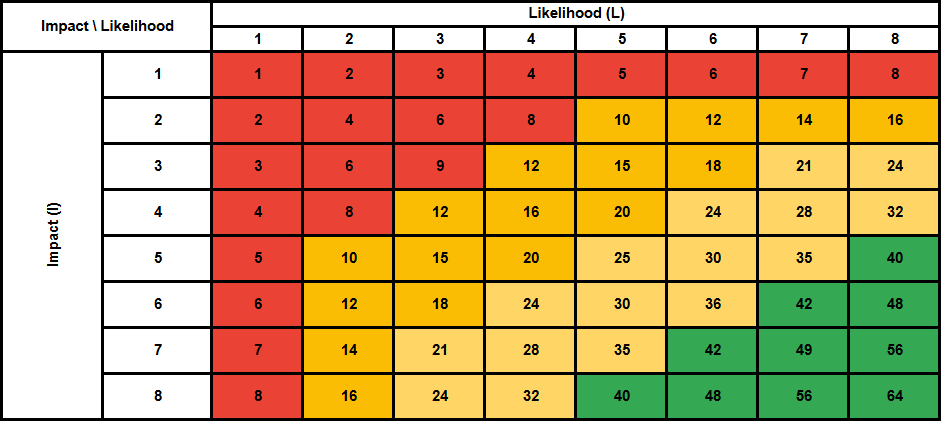
\includegraphics[width=0.9\textwidth]{Risk Assessment/Risk Assessment Matrix.png}
\caption{Risk Assessment Matrix – Systematic Evaluation Framework}
\label{fig:risk-matrix}
\end{figure}

\end{document}